\documentclass[1p]{elsarticle_modified}
%\bibliographystyle{elsarticle-num}

%\usepackage[colorlinks]{hyperref}
%\usepackage{abbrmath_seonhwa} %\Abb, \Ascr, \Acal ,\Abf, \Afrak
\usepackage{amsfonts}
\usepackage{amssymb}
\usepackage{amsmath}
\usepackage{amsthm}
\usepackage{scalefnt}
\usepackage{amsbsy}
\usepackage{kotex}
\usepackage{caption}
\usepackage{subfig}
\usepackage{color}
\usepackage{graphicx}
\usepackage{xcolor} %% white, black, red, green, blue, cyan, magenta, yellow
\usepackage{float}
\usepackage{setspace}
\usepackage{hyperref}

\usepackage{tikz}
\usetikzlibrary{arrows}

\usepackage{multirow}
\usepackage{array} % fixed length table
\usepackage{hhline}

%%%%%%%%%%%%%%%%%%%%%
\makeatletter
\renewcommand*\env@matrix[1][\arraystretch]{%
	\edef\arraystretch{#1}%
	\hskip -\arraycolsep
	\let\@ifnextchar\new@ifnextchar
	\array{*\c@MaxMatrixCols c}}
\makeatother %https://tex.stackexchange.com/questions/14071/how-can-i-increase-the-line-spacing-in-a-matrix
%%%%%%%%%%%%%%%

\usepackage[normalem]{ulem}

\newcommand{\msout}[1]{\ifmmode\text{\sout{\ensuremath{#1}}}\else\sout{#1}\fi}
%SOURCE: \msout is \stkout macro in https://tex.stackexchange.com/questions/20609/strikeout-in-math-mode

\newcommand{\cancel}[1]{
	\ifmmode
	{\color{red}\msout{#1}}
	\else
	{\color{red}\sout{#1}}
	\fi
}

\newcommand{\add}[1]{
	{\color{blue}\uwave{#1}}
}

\newcommand{\replace}[2]{
	\ifmmode
	{\color{red}\msout{#1}}{\color{blue}\uwave{#2}}
	\else
	{\color{red}\sout{#1}}{\color{blue}\uwave{#2}}
	\fi
}

\newcommand{\Sol}{\mathcal{S}} %segment
\newcommand{\D}{D} %diagram
\newcommand{\A}{\mathcal{A}} %arc


%%%%%%%%%%%%%%%%%%%%%%%%%%%%%5 test

\def\sl{\operatorname{\textup{SL}}(2,\Cbb)}
\def\psl{\operatorname{\textup{PSL}}(2,\Cbb)}
\def\quan{\mkern 1mu \triangleright \mkern 1mu}

\theoremstyle{definition}
\newtheorem{thm}{Theorem}[section]
\newtheorem{prop}[thm]{Proposition}
\newtheorem{lem}[thm]{Lemma}
\newtheorem{ques}[thm]{Question}
\newtheorem{cor}[thm]{Corollary}
\newtheorem{defn}[thm]{Definition}
\newtheorem{exam}[thm]{Example}
\newtheorem{rmk}[thm]{Remark}
\newtheorem{alg}[thm]{Algorithm}

\newcommand{\I}{\sqrt{-1}}
\begin{document}

%\begin{frontmatter}
%
%\title{Boundary parabolic representations of knots up to 8 crossings}
%
%%% Group authors per affiliation:
%\author{Yunhi Cho} 
%\address{Department of Mathematics, University of Seoul, Seoul, Korea}
%\ead{yhcho@uos.ac.kr}
%
%
%\author{Seonhwa Kim} %\fnref{s_kim}}
%\address{Center for Geometry and Physics, Institute for Basic Science, Pohang, 37673, Korea}
%\ead{ryeona17@ibs.re.kr}
%
%\author{Hyuk Kim}
%\address{Department of Mathematical Sciences, Seoul National University, Seoul 08826, Korea}
%\ead{hyukkim@snu.ac.kr}
%
%\author{Seokbeom Yoon}
%\address{Department of Mathematical Sciences, Seoul National University, Seoul, 08826,  Korea}
%\ead{sbyoon15@snu.ac.kr}
%
%\begin{abstract}
%We find all boundary parabolic representation of knots up to 8 crossings.
%
%\end{abstract}
%\begin{keyword}
%    \MSC[2010] 57M25 
%\end{keyword}
%
%\end{frontmatter}

%\linenumbers
%\tableofcontents
%
\newcommand\colored[1]{\textcolor{white}{\rule[-0.35ex]{0.8em}{1.4ex}}\kern-0.8em\color{red} #1}%
%\newcommand\colored[1]{\textcolor{white}{ #1}\kern-2.17ex	\textcolor{white}{ #1}\kern-1.81ex	\textcolor{white}{ #1}\kern-2.15ex\color{red}#1	}

{\Large $\underline{12a_{1283}~(K12a_{1283})}$}

\setlength{\tabcolsep}{10pt}
\renewcommand{\arraystretch}{1.6}
\vspace{1cm}\begin{tabular}{m{100pt}>{\centering\arraybackslash}m{274pt}}
\multirow{5}{120pt}{
	\centering
	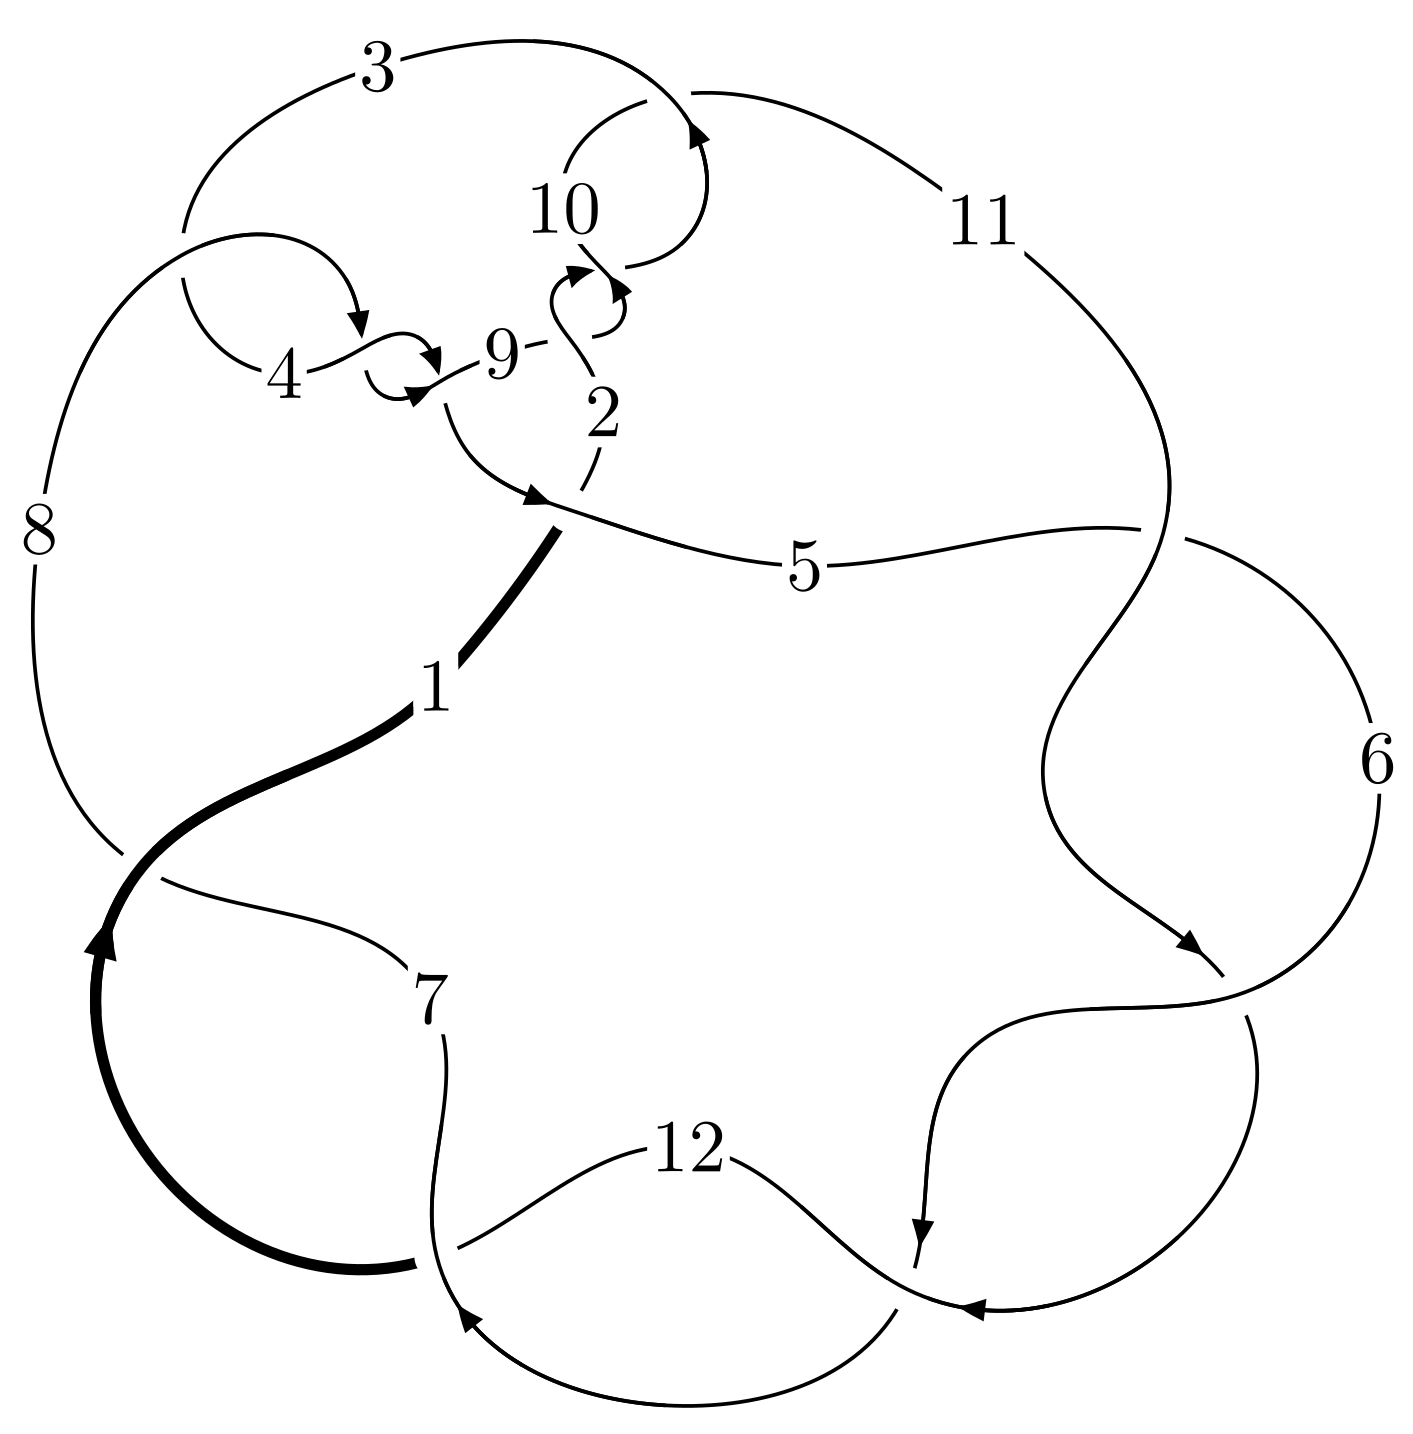
\includegraphics[width=112pt]{../../../GIT/diagram.site/Diagrams/png/2084_12a_1283.png}\\
\ \ \ A knot diagram\footnotemark}&
\allowdisplaybreaks
\textbf{Linearized knot diagam} \\
\cline{2-2}
 &
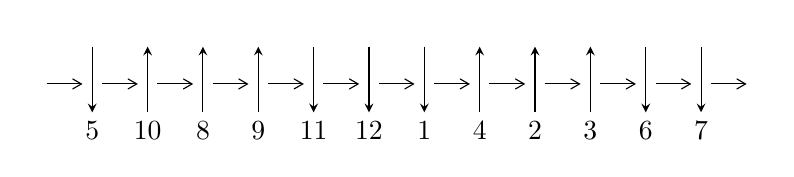
\begin{tikzpicture}[x=20pt, y=17pt]
	% nodes
	\node (C0) at (0, 0) {};
	\node (C1) at (1, 0) {};
	\node (C1U) at (1, +1) {};
	\node (C1D) at (1, -1) {5};

	\node (C2) at (2, 0) {};
	\node (C2U) at (2, +1) {};
	\node (C2D) at (2, -1) {10};

	\node (C3) at (3, 0) {};
	\node (C3U) at (3, +1) {};
	\node (C3D) at (3, -1) {8};

	\node (C4) at (4, 0) {};
	\node (C4U) at (4, +1) {};
	\node (C4D) at (4, -1) {9};

	\node (C5) at (5, 0) {};
	\node (C5U) at (5, +1) {};
	\node (C5D) at (5, -1) {11};

	\node (C6) at (6, 0) {};
	\node (C6U) at (6, +1) {};
	\node (C6D) at (6, -1) {12};

	\node (C7) at (7, 0) {};
	\node (C7U) at (7, +1) {};
	\node (C7D) at (7, -1) {1};

	\node (C8) at (8, 0) {};
	\node (C8U) at (8, +1) {};
	\node (C8D) at (8, -1) {4};

	\node (C9) at (9, 0) {};
	\node (C9U) at (9, +1) {};
	\node (C9D) at (9, -1) {2};

	\node (C10) at (10, 0) {};
	\node (C10U) at (10, +1) {};
	\node (C10D) at (10, -1) {3};

	\node (C11) at (11, 0) {};
	\node (C11U) at (11, +1) {};
	\node (C11D) at (11, -1) {6};

	\node (C12) at (12, 0) {};
	\node (C12U) at (12, +1) {};
	\node (C12D) at (12, -1) {7};
	\node (C13) at (13, 0) {};

	% arrows
	\draw[->,>={angle 60}]
	(C0) edge (C1) (C1) edge (C2) (C2) edge (C3) (C3) edge (C4) (C4) edge (C5) (C5) edge (C6) (C6) edge (C7) (C7) edge (C8) (C8) edge (C9) (C9) edge (C10) (C10) edge (C11) (C11) edge (C12) (C12) edge (C13) ;	\draw[->,>=stealth]
	(C1U) edge (C1D) (C2D) edge (C2U) (C3D) edge (C3U) (C4D) edge (C4U) (C5U) edge (C5D) (C6U) edge (C6D) (C7U) edge (C7D) (C8D) edge (C8U) (C9D) edge (C9U) (C10D) edge (C10U) (C11U) edge (C11D) (C12U) edge (C12D) ;
	\end{tikzpicture} \\
\hhline{~~} \\& 
\textbf{Solving Sequence} \\ \cline{2-2} 
 &
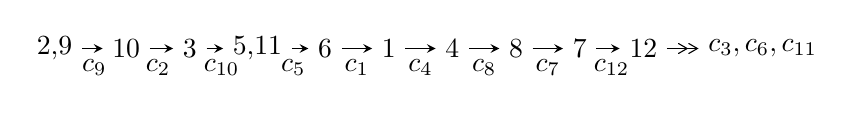
\begin{tikzpicture}[x=23pt, y=7pt]
	% node
	\node (A0) at (-1/8, 0) {2,9};
	\node (A1) at (1, 0) {10};
	\node (A2) at (2, 0) {3};
	\node (A3) at (49/16, 0) {5,11};
	\node (A4) at (33/8, 0) {6};
	\node (A5) at (41/8, 0) {1};
	\node (A6) at (49/8, 0) {4};
	\node (A7) at (57/8, 0) {8};
	\node (A8) at (65/8, 0) {7};
	\node (A9) at (73/8, 0) {12};
	\node (C1) at (1/2, -1) {$c_{9}$};
	\node (C2) at (3/2, -1) {$c_{2}$};
	\node (C3) at (5/2, -1) {$c_{10}$};
	\node (C4) at (29/8, -1) {$c_{5}$};
	\node (C5) at (37/8, -1) {$c_{1}$};
	\node (C6) at (45/8, -1) {$c_{4}$};
	\node (C7) at (53/8, -1) {$c_{8}$};
	\node (C8) at (61/8, -1) {$c_{7}$};
	\node (C9) at (69/8, -1) {$c_{12}$};
	\node (A10) at (11, 0) {$c_{3},c_{6},c_{11}$};

	% edge
	\draw[->,>=stealth]	
	(A0) edge (A1) (A1) edge (A2) (A2) edge (A3) (A3) edge (A4) (A4) edge (A5) (A5) edge (A6) (A6) edge (A7) (A7) edge (A8) (A8) edge (A9) ;
	\draw[->>,>={angle 60}]	
	(A9) edge (A10);
\end{tikzpicture} \\ 

\end{tabular} \\

\footnotetext{
The image of knot diagram is generated by the software ``\textbf{Draw programme}" developed by Andrew Bartholomew(\url{http://www.layer8.co.uk/maths/draw/index.htm\#Running-draw}), where we modified some parts for our purpose(\url{https://github.com/CATsTAILs/LinksPainter}).
}\phantom \\ \newline 
\centering \textbf{Ideals for irreducible components\footnotemark of $X_{\text{par}}$} 
 
\begin{align*}
I^u_{1}&=\langle 
b- u,\;- u^{18}+u^{17}+\cdots+4 a-13 u,\;u^{19}- u^{18}+\cdots- u-1\rangle \\
I^u_{2}&=\langle 
538 u^{23}+1753 u^{22}+\cdots+3334 b+10456,\;432 u^{23}+12271 u^{22}+\cdots+23338 a+126536,\\
\phantom{I^u_{2}}&\phantom{= \langle  }u^{24}-10 u^{22}+\cdots-16 u-7\rangle \\
I^u_{3}&=\langle 
b-1,\;a^2-3,\;u+1\rangle \\
I^u_{4}&=\langle 
b-1,\;a,\;u+1\rangle \\
I^u_{5}&=\langle 
b,\;a-1,\;u-1\rangle \\
I^u_{6}&=\langle 
b+1,\;a-1,\;u-1\rangle \\
I^u_{7}&=\langle 
b+1,\;a+1,\;u-1\rangle \\
\\
I^v_{1}&=\langle 
a,\;b-1,\;v+1\rangle \\
\end{align*}
\raggedright * 8 irreducible components of $\dim_{\mathbb{C}}=0$, with total 50 representations.\\
\footnotetext{All coefficients of polynomials are rational numbers. But the coefficients are sometimes approximated in decimal forms when there is not enough margin.}
\newpage
\renewcommand{\arraystretch}{1}
\centering \section*{I. $I^u_{1}= \langle b- u,\;- u^{18}+u^{17}+\cdots+4 a-13 u,\;u^{19}- u^{18}+\cdots- u-1 \rangle$}
\flushleft \textbf{(i) Arc colorings}\\
\begin{tabular}{m{7pt} m{180pt} m{7pt} m{180pt} }
\flushright $a_{2}=$&$\begin{pmatrix}0\\u\end{pmatrix}$ \\
\flushright $a_{9}=$&$\begin{pmatrix}1\\0\end{pmatrix}$ \\
\flushright $a_{10}=$&$\begin{pmatrix}1\\- u^2\end{pmatrix}$ \\
\flushright $a_{3}=$&$\begin{pmatrix}u\\- u^3+u\end{pmatrix}$ \\
\flushright $a_{5}=$&$\begin{pmatrix}\frac{1}{4} u^{18}-\frac{1}{4} u^{17}+\cdots+\frac{1}{4} u^2+\frac{13}{4} u\\u\end{pmatrix}$ \\
\flushright $a_{11}=$&$\begin{pmatrix}- u^2+1\\u^4-2 u^2\end{pmatrix}$ \\
\flushright $a_{6}=$&$\begin{pmatrix}\frac{1}{4} u^{18}-\frac{1}{4} u^{17}+\cdots+\frac{1}{4} u^2+\frac{9}{4} u\\\frac{1}{4} u^{18}-\frac{1}{4} u^{17}+\cdots+\frac{1}{4} u^2+\frac{5}{4} u\end{pmatrix}$ \\
\flushright $a_{1}=$&$\begin{pmatrix}-\frac{1}{4} u^{17}-\frac{1}{4} u^{16}+\cdots+\frac{1}{4} u-\frac{1}{4}\\\frac{1}{4} u^{18}-\frac{1}{4} u^{17}+\cdots+\frac{1}{4} u^2+\frac{5}{4} u\end{pmatrix}$ \\
\flushright $a_{4}=$&$\begin{pmatrix}\frac{1}{4} u^{18}-\frac{1}{4} u^{17}+\cdots+\frac{1}{4} u^2+\frac{9}{4} u\\u\end{pmatrix}$ \\
\flushright $a_{8}=$&$\begin{pmatrix}\frac{1}{4} u^{17}-\frac{1}{4} u^{16}+\cdots+\frac{1}{4} u+\frac{5}{4}\\u^2\end{pmatrix}$ \\
\flushright $a_{7}=$&$\begin{pmatrix}\frac{1}{2} u^{18}-\frac{3}{2} u^{17}+\cdots-\frac{1}{2} u-\frac{1}{2}\\\frac{1}{4} u^{18}-\frac{11}{4} u^{16}+\cdots-\frac{1}{2} u^2-\frac{1}{4}\end{pmatrix}$ \\
\flushright $a_{12}=$&$\begin{pmatrix}-\frac{1}{4} u^{18}-\frac{1}{4} u^{17}+\cdots-\frac{1}{4} u+1\\-\frac{1}{4} u^{18}+\frac{1}{2} u^{17}+\cdots+\frac{1}{2} u+\frac{3}{4}\end{pmatrix}$\\&\end{tabular}
\flushleft \textbf{(ii) Obstruction class $= -1$}\\~\\
\flushleft \textbf{(iii) Cusp Shapes $= -\frac{3}{2} u^{18}+\frac{5}{2} u^{17}+17 u^{16}-\frac{51}{2} u^{15}-81 u^{14}+104 u^{13}+206 u^{12}-\frac{411}{2} u^{11}-\frac{583}{2} u^{10}+\frac{351}{2} u^9+215 u^8-\frac{9}{2} u^7-\frac{149}{2} u^6-\frac{103}{2} u^5+36 u^4-\frac{29}{2} u^3-\frac{59}{2} u^2+\frac{15}{2} u$}\\~\\
\newpage\renewcommand{\arraystretch}{1}
\flushleft \textbf{(iv) u-Polynomials at the component}\newline \\
\begin{tabular}{m{50pt}|m{274pt}}
Crossings & \hspace{64pt}u-Polynomials at each crossing \\
\hline $$\begin{aligned}c_{1}\end{aligned}$$&$\begin{aligned}
&u^{19}+15 u^{18}+\cdots+1586 u+218
\end{aligned}$\\
\hline $$\begin{aligned}c_{2},c_{3},c_{4}\\c_{8},c_{9},c_{10}\end{aligned}$$&$\begin{aligned}
&u^{19}+u^{18}+\cdots- u+1
\end{aligned}$\\
\hline $$\begin{aligned}c_{5},c_{6},c_{7}\\c_{11},c_{12}\end{aligned}$$&$\begin{aligned}
&u^{19}+3 u^{18}+\cdots-6 u-2
\end{aligned}$\\
\hline
\end{tabular}\\~\\
\newpage\renewcommand{\arraystretch}{1}
\flushleft \textbf{(v) Riley Polynomials at the component}\newline \\
\begin{tabular}{m{50pt}|m{274pt}}
Crossings & \hspace{64pt}Riley Polynomials at each crossing \\
\hline $$\begin{aligned}c_{1}\end{aligned}$$&$\begin{aligned}
&y^{19}- y^{18}+\cdots+65512 y-47524
\end{aligned}$\\
\hline $$\begin{aligned}c_{2},c_{3},c_{4}\\c_{8},c_{9},c_{10}\end{aligned}$$&$\begin{aligned}
&y^{19}-23 y^{18}+\cdots+y-1
\end{aligned}$\\
\hline $$\begin{aligned}c_{5},c_{6},c_{7}\\c_{11},c_{12}\end{aligned}$$&$\begin{aligned}
&y^{19}-25 y^{18}+\cdots-24 y-4
\end{aligned}$\\
\hline
\end{tabular}\\~\\
\newpage\flushleft \textbf{(vi) Complex Volumes and Cusp Shapes}
$$\begin{array}{c|c|c}  
\text{Solutions to }I^u_{1}& \I (\text{vol} + \sqrt{-1}CS) & \text{Cusp shape}\\
 \hline 
\begin{aligned}
u &= -0.310639 + 0.700279 I \\
a &= -0.43101 + 1.74263 I \\
b &= -0.310639 + 0.700279 I\end{aligned}
 & -12.66640 - 3.70859 I & -6.97096 + 4.51080 I \\ \hline\begin{aligned}
u &= -0.310639 - 0.700279 I \\
a &= -0.43101 - 1.74263 I \\
b &= -0.310639 - 0.700279 I\end{aligned}
 & -12.66640 + 3.70859 I & -6.97096 - 4.51080 I \\ \hline\begin{aligned}
u &= -1.34431\phantom{ +0.000000I} \\
a &= \phantom{-}1.98662\phantom{ +0.000000I} \\
b &= -1.34431\phantom{ +0.000000I}\end{aligned}
 & -7.55334\phantom{ +0.000000I} & \phantom{-}2.37220\phantom{ +0.000000I} \\ \hline\begin{aligned}
u &= \phantom{-}0.264676 + 0.585091 I \\
a &= \phantom{-}0.44609 + 1.54901 I \\
b &= \phantom{-}0.264676 + 0.585091 I\end{aligned}
 & -3.30479 + 2.71809 I & -7.05035 - 6.50802 I \\ \hline\begin{aligned}
u &= \phantom{-}0.264676 - 0.585091 I \\
a &= \phantom{-}0.44609 - 1.54901 I \\
b &= \phantom{-}0.264676 - 0.585091 I\end{aligned}
 & -3.30479 - 2.71809 I & -7.05035 + 6.50802 I \\ \hline\begin{aligned}
u &= -0.583241\phantom{ +0.000000I} \\
a &= -2.35110\phantom{ +0.000000I} \\
b &= -0.583241\phantom{ +0.000000I}\end{aligned}
 & -11.3004\phantom{ +0.000000I} & -5.80070\phantom{ +0.000000I} \\ \hline\begin{aligned}
u &= \phantom{-}1.47018\phantom{ +0.000000I} \\
a &= -1.06148\phantom{ +0.000000I} \\
b &= \phantom{-}1.47018\phantom{ +0.000000I}\end{aligned}
 & \phantom{-}3.59702\phantom{ +0.000000I} & \phantom{-}2.15400\phantom{ +0.000000I} \\ \hline\begin{aligned}
u &= \phantom{-}1.48891 + 0.35458 I \\
a &= -0.245253 + 1.382770 I \\
b &= \phantom{-}1.48891 + 0.35458 I\end{aligned}
 & -1.12008 + 11.80290 I & \phantom{-}0.70242 - 5.53182 I \\ \hline\begin{aligned}
u &= \phantom{-}1.48891 - 0.35458 I \\
a &= -0.245253 - 1.382770 I \\
b &= \phantom{-}1.48891 - 0.35458 I\end{aligned}
 & -1.12008 - 11.80290 I & \phantom{-}0.70242 + 5.53182 I \\ \hline\begin{aligned}
u &= -1.52435 + 0.16917 I \\
a &= \phantom{-}0.597354 + 0.752907 I \\
b &= -1.52435 + 0.16917 I\end{aligned}
 & \phantom{-}10.36490 - 2.09930 I & \phantom{-}4.61522 - 0.98931 I\\
 \hline 
 \end{array}$$\newpage$$\begin{array}{c|c|c}  
\text{Solutions to }I^u_{1}& \I (\text{vol} + \sqrt{-1}CS) & \text{Cusp shape}\\
 \hline 
\begin{aligned}
u &= -1.52435 - 0.16917 I \\
a &= \phantom{-}0.597354 - 0.752907 I \\
b &= -1.52435 - 0.16917 I\end{aligned}
 & \phantom{-}10.36490 + 2.09930 I & \phantom{-}4.61522 + 0.98931 I \\ \hline\begin{aligned}
u &= -1.50399 + 0.30349 I \\
a &= \phantom{-}0.345723 + 1.228060 I \\
b &= -1.50399 + 0.30349 I\end{aligned}
 & \phantom{-}8.30594 - 9.64872 I & \phantom{-}2.30074 + 6.54307 I \\ \hline\begin{aligned}
u &= -1.50399 - 0.30349 I \\
a &= \phantom{-}0.345723 - 1.228060 I \\
b &= -1.50399 - 0.30349 I\end{aligned}
 & \phantom{-}8.30594 + 9.64872 I & \phantom{-}2.30074 - 6.54307 I \\ \hline\begin{aligned}
u &= \phantom{-}1.54004\phantom{ +0.000000I} \\
a &= -0.705382\phantom{ +0.000000I} \\
b &= \phantom{-}1.54004\phantom{ +0.000000I}\end{aligned}
 & \phantom{-}3.55474\phantom{ +0.000000I} & \phantom{-}2.45220\phantom{ +0.000000I} \\ \hline\begin{aligned}
u &= \phantom{-}1.52397 + 0.24269 I \\
a &= -0.439996 + 1.008280 I \\
b &= \phantom{-}1.52397 + 0.24269 I\end{aligned}
 & \phantom{-}11.80370 + 6.00675 I & \phantom{-}6.85446 - 4.30060 I \\ \hline\begin{aligned}
u &= \phantom{-}1.52397 - 0.24269 I \\
a &= -0.439996 - 1.008280 I \\
b &= \phantom{-}1.52397 - 0.24269 I\end{aligned}
 & \phantom{-}11.80370 - 6.00675 I & \phantom{-}6.85446 + 4.30060 I \\ \hline\begin{aligned}
u &= \phantom{-}0.440690\phantom{ +0.000000I} \\
a &= \phantom{-}1.53450\phantom{ +0.000000I} \\
b &= \phantom{-}0.440690\phantom{ +0.000000I}\end{aligned}
 & -1.88440\phantom{ +0.000000I} & -3.40050\phantom{ +0.000000I} \\ \hline\begin{aligned}
u &= -0.200256 + 0.361761 I \\
a &= -0.474490 + 1.061500 I \\
b &= -0.200256 + 0.361761 I\end{aligned}
 & -0.010314 - 0.815704 I & -0.34015 + 8.34541 I \\ \hline\begin{aligned}
u &= -0.200256 - 0.361761 I \\
a &= -0.474490 - 1.061500 I \\
b &= -0.200256 - 0.361761 I\end{aligned}
 & -0.010314 + 0.815704 I & -0.34015 - 8.34541 I\\
 \hline 
 \end{array}$$\newpage\newpage\renewcommand{\arraystretch}{1}
\centering \section*{II. $I^u_{2}= \langle 538 u^{23}+1753 u^{22}+\cdots+3334 b+10456,\;432 u^{23}+12271 u^{22}+\cdots+23338 a+126536,\;u^{24}-10 u^{22}+\cdots-16 u-7 \rangle$}
\flushleft \textbf{(i) Arc colorings}\\
\begin{tabular}{m{7pt} m{180pt} m{7pt} m{180pt} }
\flushright $a_{2}=$&$\begin{pmatrix}0\\u\end{pmatrix}$ \\
\flushright $a_{9}=$&$\begin{pmatrix}1\\0\end{pmatrix}$ \\
\flushright $a_{10}=$&$\begin{pmatrix}1\\- u^2\end{pmatrix}$ \\
\flushright $a_{3}=$&$\begin{pmatrix}u\\- u^3+u\end{pmatrix}$ \\
\flushright $a_{5}=$&$\begin{pmatrix}-0.0185106 u^{23}-0.525795 u^{22}+\cdots-3.14153 u-5.42189\\-0.161368 u^{23}-0.525795 u^{22}+\cdots-5.71296 u-3.13617\end{pmatrix}$ \\
\flushright $a_{11}=$&$\begin{pmatrix}- u^2+1\\u^4-2 u^2\end{pmatrix}$ \\
\flushright $a_{6}=$&$\begin{pmatrix}-0.0101123 u^{23}-0.227055 u^{22}+\cdots-0.0356500 u-2.14714\\-0.155369 u^{23}-0.0266947 u^{22}+\cdots-0.708758 u-1.08278\end{pmatrix}$ \\
\flushright $a_{1}=$&$\begin{pmatrix}0.166252 u^{23}+0.0464907 u^{22}+\cdots+1.68781 u-4.87750\\0.184763 u^{23}+0.572286 u^{22}+\cdots+5.82933 u+0.544391\end{pmatrix}$ \\
\flushright $a_{4}=$&$\begin{pmatrix}\frac{1}{7} u^{23}-\frac{10}{7} u^{21}+\cdots+\frac{18}{7} u-\frac{16}{7}\\-0.161368 u^{23}-0.525795 u^{22}+\cdots-5.71296 u-3.13617\end{pmatrix}$ \\
\flushright $a_{8}=$&$\begin{pmatrix}-0.448025 u^{23}-0.161368 u^{22}+\cdots-3.84219 u+2.45544\\0.525795 u^{23}+0.346131 u^{22}+\cdots+5.71806 u+2.12957\end{pmatrix}$ \\
\flushright $a_{7}=$&$\begin{pmatrix}-0.0533893 u^{23}-0.0419916 u^{22}+\cdots+0.862627 u-5.17516\\-0.0929814 u^{23}+0.263947 u^{22}+\cdots+4.43491 u-0.327534\end{pmatrix}$ \\
\flushright $a_{12}=$&$\begin{pmatrix}-0.268960 u^{23}-0.363227 u^{22}+\cdots-3.56684 u+3.09911\\0.134673 u^{23}+0.00479904 u^{22}+\cdots-2.85573 u+0.548590\end{pmatrix}$\\&\end{tabular}
\flushleft \textbf{(ii) Obstruction class $= -1$}\\~\\
\flushleft \textbf{(iii) Cusp Shapes $= -\frac{654}{1667} u^{23}-\frac{3736}{1667} u^{22}+\cdots-\frac{38132}{1667} u-\frac{26158}{1667}$}\\~\\
\newpage\renewcommand{\arraystretch}{1}
\flushleft \textbf{(iv) u-Polynomials at the component}\newline \\
\begin{tabular}{m{50pt}|m{274pt}}
Crossings & \hspace{64pt}u-Polynomials at each crossing \\
\hline $$\begin{aligned}c_{1}\end{aligned}$$&$\begin{aligned}
&(u^{12}-4 u^{11}+\cdots-6 u+1)^{2}
\end{aligned}$\\
\hline $$\begin{aligned}c_{2},c_{3},c_{4}\\c_{8},c_{9},c_{10}\end{aligned}$$&$\begin{aligned}
&u^{24}-10 u^{22}+\cdots+16 u-7
\end{aligned}$\\
\hline $$\begin{aligned}c_{5},c_{6},c_{7}\\c_{11},c_{12}\end{aligned}$$&$\begin{aligned}
&(u^{12}-2 u^{11}+\cdots-4 u+1)^{2}
\end{aligned}$\\
\hline
\end{tabular}\\~\\
\newpage\renewcommand{\arraystretch}{1}
\flushleft \textbf{(v) Riley Polynomials at the component}\newline \\
\begin{tabular}{m{50pt}|m{274pt}}
Crossings & \hspace{64pt}Riley Polynomials at each crossing \\
\hline $$\begin{aligned}c_{1}\end{aligned}$$&$\begin{aligned}
&(y^{12}+8 y^{11}+\cdots-14 y+1)^{2}
\end{aligned}$\\
\hline $$\begin{aligned}c_{2},c_{3},c_{4}\\c_{8},c_{9},c_{10}\end{aligned}$$&$\begin{aligned}
&y^{24}-20 y^{23}+\cdots-508 y+49
\end{aligned}$\\
\hline $$\begin{aligned}c_{5},c_{6},c_{7}\\c_{11},c_{12}\end{aligned}$$&$\begin{aligned}
&(y^{12}-16 y^{11}+\cdots-6 y+1)^{2}
\end{aligned}$\\
\hline
\end{tabular}\\~\\
\newpage\flushleft \textbf{(vi) Complex Volumes and Cusp Shapes}
$$\begin{array}{c|c|c}  
\text{Solutions to }I^u_{2}& \I (\text{vol} + \sqrt{-1}CS) & \text{Cusp shape}\\
 \hline 
\begin{aligned}
u &= -0.358425 + 0.917120 I \\
a &= \phantom{-}1.06378 - 1.20789 I \\
b &= \phantom{-}1.43345 - 0.26200 I\end{aligned}
 & -7.05914 - 7.20360 I & -2.08749 + 4.71657 I \\ \hline\begin{aligned}
u &= -0.358425 - 0.917120 I \\
a &= \phantom{-}1.06378 + 1.20789 I \\
b &= \phantom{-}1.43345 + 0.26200 I\end{aligned}
 & -7.05914 + 7.20360 I & -2.08749 - 4.71657 I \\ \hline\begin{aligned}
u &= \phantom{-}0.726659 + 0.612159 I \\
a &= -0.556760 - 0.649993 I \\
b &= -1.361680 + 0.028095 I\end{aligned}
 & \phantom{-}3.08210 - 0.49850 I & \phantom{-}1.36863 + 1.38008 I \\ \hline\begin{aligned}
u &= \phantom{-}0.726659 - 0.612159 I \\
a &= -0.556760 + 0.649993 I \\
b &= -1.361680 - 0.028095 I\end{aligned}
 & \phantom{-}3.08210 + 0.49850 I & \phantom{-}1.36863 - 1.38008 I \\ \hline\begin{aligned}
u &= \phantom{-}0.421897 + 0.830088 I \\
a &= -0.92080 - 1.15289 I \\
b &= -1.40739 - 0.19551 I\end{aligned}
 & \phantom{-}2.05779 + 5.52285 I & -0.56374 - 6.48307 I \\ \hline\begin{aligned}
u &= \phantom{-}0.421897 - 0.830088 I \\
a &= -0.92080 + 1.15289 I \\
b &= -1.40739 + 0.19551 I\end{aligned}
 & \phantom{-}2.05779 - 5.52285 I & -0.56374 + 6.48307 I \\ \hline\begin{aligned}
u &= -0.539453 + 0.732545 I \\
a &= \phantom{-}0.737853 - 0.986740 I \\
b &= \phantom{-}1.389660 - 0.101631 I\end{aligned}
 & \phantom{-}5.05906 - 2.46907 I & \phantom{-}5.52253 + 3.95252 I \\ \hline\begin{aligned}
u &= -0.539453 - 0.732545 I \\
a &= \phantom{-}0.737853 + 0.986740 I \\
b &= \phantom{-}1.389660 + 0.101631 I\end{aligned}
 & \phantom{-}5.05906 + 2.46907 I & \phantom{-}5.52253 - 3.95252 I \\ \hline\begin{aligned}
u &= -0.914759 + 0.672614 I \\
a &= \phantom{-}0.716633 - 0.381724 I \\
b &= \phantom{-}1.42619 + 0.14001 I\end{aligned}
 & -5.38423 + 1.70959 I & \phantom{-}0.128193 - 0.167200 I \\ \hline\begin{aligned}
u &= -0.914759 - 0.672614 I \\
a &= \phantom{-}0.716633 + 0.381724 I \\
b &= \phantom{-}1.42619 - 0.14001 I\end{aligned}
 & -5.38423 - 1.70959 I & \phantom{-}0.128193 + 0.167200 I\\
 \hline 
 \end{array}$$\newpage$$\begin{array}{c|c|c}  
\text{Solutions to }I^u_{2}& \I (\text{vol} + \sqrt{-1}CS) & \text{Cusp shape}\\
 \hline 
\begin{aligned}
u &= -1.14845\phantom{ +0.000000I} \\
a &= -0.192638\phantom{ +0.000000I} \\
b &= \phantom{-}0.678097\phantom{ +0.000000I}\end{aligned}
 & \phantom{-}2.62918\phantom{ +0.000000I} & -3.06920\phantom{ +0.000000I} \\ \hline\begin{aligned}
u &= \phantom{-}0.678097\phantom{ +0.000000I} \\
a &= \phantom{-}0.326261\phantom{ +0.000000I} \\
b &= -1.14845\phantom{ +0.000000I}\end{aligned}
 & \phantom{-}2.62918\phantom{ +0.000000I} & -3.06920\phantom{ +0.000000I} \\ \hline\begin{aligned}
u &= -1.361680 + 0.028095 I \\
a &= -0.007416 + 0.597014 I \\
b &= \phantom{-}0.726659 + 0.612159 I\end{aligned}
 & \phantom{-}3.08210 - 0.49850 I & \phantom{-}1.36863 + 1.38008 I \\ \hline\begin{aligned}
u &= -1.361680 - 0.028095 I \\
a &= -0.007416 - 0.597014 I \\
b &= \phantom{-}0.726659 - 0.612159 I\end{aligned}
 & \phantom{-}3.08210 + 0.49850 I & \phantom{-}1.36863 - 1.38008 I \\ \hline\begin{aligned}
u &= \phantom{-}1.389660 + 0.101631 I \\
a &= \phantom{-}0.176320 - 0.784892 I \\
b &= -0.539453 - 0.732545 I\end{aligned}
 & \phantom{-}5.05906 + 2.46907 I & \phantom{-}5.52253 - 3.95252 I \\ \hline\begin{aligned}
u &= \phantom{-}1.389660 - 0.101631 I \\
a &= \phantom{-}0.176320 + 0.784892 I \\
b &= -0.539453 + 0.732545 I\end{aligned}
 & \phantom{-}5.05906 - 2.46907 I & \phantom{-}5.52253 + 3.95252 I \\ \hline\begin{aligned}
u &= -0.580967 + 0.112101 I \\
a &= -2.24045 - 0.43231 I \\
b &= -0.580967 - 0.112101 I\end{aligned}
 & -11.2998\phantom{ +0.000000I} & -5.66710 + 0. I\phantom{ +0.000000I} \\ \hline\begin{aligned}
u &= -0.580967 - 0.112101 I \\
a &= -2.24045 + 0.43231 I \\
b &= -0.580967 + 0.112101 I\end{aligned}
 & -11.2998\phantom{ +0.000000I} & -5.66710 + 0. I\phantom{ +0.000000I} \\ \hline\begin{aligned}
u &= -1.40739 + 0.19551 I \\
a &= -0.275184 - 0.926925 I \\
b &= \phantom{-}0.421897 - 0.830088 I\end{aligned}
 & \phantom{-}2.05779 - 5.52285 I & -0.56374 + 6.48307 I \\ \hline\begin{aligned}
u &= -1.40739 - 0.19551 I \\
a &= -0.275184 + 0.926925 I \\
b &= \phantom{-}0.421897 + 0.830088 I\end{aligned}
 & \phantom{-}2.05779 + 5.52285 I & -0.56374 - 6.48307 I\\
 \hline 
 \end{array}$$\newpage$$\begin{array}{c|c|c}  
\text{Solutions to }I^u_{2}& \I (\text{vol} + \sqrt{-1}CS) & \text{Cusp shape}\\
 \hline 
\begin{aligned}
u &= \phantom{-}1.42619 + 0.14001 I \\
a &= -0.220284 + 0.604438 I \\
b &= -0.914759 + 0.672614 I\end{aligned}
 & -5.38423 + 1.70959 I & \phantom{-}0.128193 - 0.167200 I \\ \hline\begin{aligned}
u &= \phantom{-}1.42619 - 0.14001 I \\
a &= -0.220284 - 0.604438 I \\
b &= -0.914759 - 0.672614 I\end{aligned}
 & -5.38423 - 1.70959 I & \phantom{-}0.128193 + 0.167200 I \\ \hline\begin{aligned}
u &= \phantom{-}1.43345 + 0.26200 I \\
a &= \phantom{-}0.316640 - 1.040500 I \\
b &= -0.358425 - 0.917120 I\end{aligned}
 & -7.05914 + 7.20360 I & -2.08749 - 4.71657 I \\ \hline\begin{aligned}
u &= \phantom{-}1.43345 - 0.26200 I \\
a &= \phantom{-}0.316640 + 1.040500 I \\
b &= -0.358425 + 0.917120 I\end{aligned}
 & -7.05914 - 7.20360 I & -2.08749 + 4.71657 I\\
 \hline 
 \end{array}$$\newpage\newpage\renewcommand{\arraystretch}{1}
\centering \section*{III. $I^u_{3}= \langle b-1,\;a^2-3,\;u+1 \rangle$}
\flushleft \textbf{(i) Arc colorings}\\
\begin{tabular}{m{7pt} m{180pt} m{7pt} m{180pt} }
\flushright $a_{2}=$&$\begin{pmatrix}0\\-1\end{pmatrix}$ \\
\flushright $a_{9}=$&$\begin{pmatrix}1\\0\end{pmatrix}$ \\
\flushright $a_{10}=$&$\begin{pmatrix}1\\-1\end{pmatrix}$ \\
\flushright $a_{3}=$&$\begin{pmatrix}-1\\0\end{pmatrix}$ \\
\flushright $a_{5}=$&$\begin{pmatrix}a\\1\end{pmatrix}$ \\
\flushright $a_{11}=$&$\begin{pmatrix}0\\-1\end{pmatrix}$ \\
\flushright $a_{6}=$&$\begin{pmatrix}a\\a+1\end{pmatrix}$ \\
\flushright $a_{1}=$&$\begin{pmatrix}-3\\- a-1\end{pmatrix}$ \\
\flushright $a_{4}=$&$\begin{pmatrix}a-1\\1\end{pmatrix}$ \\
\flushright $a_{8}=$&$\begin{pmatrix}a\\1\end{pmatrix}$ \\
\flushright $a_{7}=$&$\begin{pmatrix}-2 a\\- a-2\end{pmatrix}$ \\
\flushright $a_{12}=$&$\begin{pmatrix}3\\a+2\end{pmatrix}$\\&\end{tabular}
\flushleft \textbf{(ii) Obstruction class $= 1$}\\~\\
\flushleft \textbf{(iii) Cusp Shapes $= 0$}\\~\\
\newpage\renewcommand{\arraystretch}{1}
\flushleft \textbf{(iv) u-Polynomials at the component}\newline \\
\begin{tabular}{m{50pt}|m{274pt}}
Crossings & \hspace{64pt}u-Polynomials at each crossing \\
\hline $$\begin{aligned}c_{1},c_{5},c_{6}\\c_{7},c_{11},c_{12}\end{aligned}$$&$\begin{aligned}
&u^2-3
\end{aligned}$\\
\hline $$\begin{aligned}c_{2},c_{8}\end{aligned}$$&$\begin{aligned}
&(u-1)^2
\end{aligned}$\\
\hline $$\begin{aligned}c_{3},c_{4},c_{9}\\c_{10}\end{aligned}$$&$\begin{aligned}
&(u+1)^2
\end{aligned}$\\
\hline
\end{tabular}\\~\\
\newpage\renewcommand{\arraystretch}{1}
\flushleft \textbf{(v) Riley Polynomials at the component}\newline \\
\begin{tabular}{m{50pt}|m{274pt}}
Crossings & \hspace{64pt}Riley Polynomials at each crossing \\
\hline $$\begin{aligned}c_{1},c_{5},c_{6}\\c_{7},c_{11},c_{12}\end{aligned}$$&$\begin{aligned}
&(y-3)^2
\end{aligned}$\\
\hline $$\begin{aligned}c_{2},c_{3},c_{4}\\c_{8},c_{9},c_{10}\end{aligned}$$&$\begin{aligned}
&(y-1)^2
\end{aligned}$\\
\hline
\end{tabular}\\~\\
\newpage\flushleft \textbf{(vi) Complex Volumes and Cusp Shapes}
$$\begin{array}{c|c|c}  
\text{Solutions to }I^u_{3}& \I (\text{vol} + \sqrt{-1}CS) & \text{Cusp shape}\\
 \hline 
\begin{aligned}
u &= -1.00000\phantom{ +0.000000I} \\
a &= \phantom{-}1.73205\phantom{ +0.000000I} \\
b &= \phantom{-}1.00000\phantom{ +0.000000I}\end{aligned}
 & -9.86960\phantom{ +0.000000I} & \phantom{-0.000000 } 0 \\ \hline\begin{aligned}
u &= -1.00000\phantom{ +0.000000I} \\
a &= -1.73205\phantom{ +0.000000I} \\
b &= \phantom{-}1.00000\phantom{ +0.000000I}\end{aligned}
 & -9.86960\phantom{ +0.000000I} & \phantom{-0.000000 } 0\\
 \hline 
 \end{array}$$\newpage\newpage\renewcommand{\arraystretch}{1}
\centering \section*{IV. $I^u_{4}= \langle b-1,\;a,\;u+1 \rangle$}
\flushleft \textbf{(i) Arc colorings}\\
\begin{tabular}{m{7pt} m{180pt} m{7pt} m{180pt} }
\flushright $a_{2}=$&$\begin{pmatrix}0\\-1\end{pmatrix}$ \\
\flushright $a_{9}=$&$\begin{pmatrix}1\\0\end{pmatrix}$ \\
\flushright $a_{10}=$&$\begin{pmatrix}1\\-1\end{pmatrix}$ \\
\flushright $a_{3}=$&$\begin{pmatrix}-1\\0\end{pmatrix}$ \\
\flushright $a_{5}=$&$\begin{pmatrix}0\\1\end{pmatrix}$ \\
\flushright $a_{11}=$&$\begin{pmatrix}0\\-1\end{pmatrix}$ \\
\flushright $a_{6}=$&$\begin{pmatrix}0\\1\end{pmatrix}$ \\
\flushright $a_{1}=$&$\begin{pmatrix}0\\-1\end{pmatrix}$ \\
\flushright $a_{4}=$&$\begin{pmatrix}-1\\1\end{pmatrix}$ \\
\flushright $a_{8}=$&$\begin{pmatrix}0\\1\end{pmatrix}$ \\
\flushright $a_{7}=$&$\begin{pmatrix}0\\1\end{pmatrix}$ \\
\flushright $a_{12}=$&$\begin{pmatrix}0\\-1\end{pmatrix}$\\&\end{tabular}
\flushleft \textbf{(ii) Obstruction class $= 1$}\\~\\
\flushleft \textbf{(iii) Cusp Shapes $= 12$}\\~\\
\newpage\renewcommand{\arraystretch}{1}
\flushleft \textbf{(iv) u-Polynomials at the component}\newline \\
\begin{tabular}{m{50pt}|m{274pt}}
Crossings & \hspace{64pt}u-Polynomials at each crossing \\
\hline $$\begin{aligned}c_{1},c_{5},c_{6}\\c_{7},c_{11},c_{12}\end{aligned}$$&$\begin{aligned}
&u
\end{aligned}$\\
\hline $$\begin{aligned}c_{2},c_{8}\end{aligned}$$&$\begin{aligned}
&u-1
\end{aligned}$\\
\hline $$\begin{aligned}c_{3},c_{4},c_{9}\\c_{10}\end{aligned}$$&$\begin{aligned}
&u+1
\end{aligned}$\\
\hline
\end{tabular}\\~\\
\newpage\renewcommand{\arraystretch}{1}
\flushleft \textbf{(v) Riley Polynomials at the component}\newline \\
\begin{tabular}{m{50pt}|m{274pt}}
Crossings & \hspace{64pt}Riley Polynomials at each crossing \\
\hline $$\begin{aligned}c_{1},c_{5},c_{6}\\c_{7},c_{11},c_{12}\end{aligned}$$&$\begin{aligned}
&y
\end{aligned}$\\
\hline $$\begin{aligned}c_{2},c_{3},c_{4}\\c_{8},c_{9},c_{10}\end{aligned}$$&$\begin{aligned}
&y-1
\end{aligned}$\\
\hline
\end{tabular}\\~\\
\newpage\flushleft \textbf{(vi) Complex Volumes and Cusp Shapes}
$$\begin{array}{c|c|c}  
\text{Solutions to }I^u_{4}& \I (\text{vol} + \sqrt{-1}CS) & \text{Cusp shape}\\
 \hline 
\begin{aligned}
u &= -1.00000\phantom{ +0.000000I} \\
a &= \phantom{-0.000000 } 0 \\
b &= \phantom{-}1.00000\phantom{ +0.000000I}\end{aligned}
 & \phantom{-}3.28987\phantom{ +0.000000I} & \phantom{-}12.0000\phantom{ +0.000000I}\\
 \hline 
 \end{array}$$\newpage\newpage\renewcommand{\arraystretch}{1}
\centering \section*{V. $I^u_{5}= \langle b,\;a-1,\;u-1 \rangle$}
\flushleft \textbf{(i) Arc colorings}\\
\begin{tabular}{m{7pt} m{180pt} m{7pt} m{180pt} }
\flushright $a_{2}=$&$\begin{pmatrix}0\\1\end{pmatrix}$ \\
\flushright $a_{9}=$&$\begin{pmatrix}1\\0\end{pmatrix}$ \\
\flushright $a_{10}=$&$\begin{pmatrix}1\\-1\end{pmatrix}$ \\
\flushright $a_{3}=$&$\begin{pmatrix}1\\0\end{pmatrix}$ \\
\flushright $a_{5}=$&$\begin{pmatrix}1\\0\end{pmatrix}$ \\
\flushright $a_{11}=$&$\begin{pmatrix}0\\-1\end{pmatrix}$ \\
\flushright $a_{6}=$&$\begin{pmatrix}1\\1\end{pmatrix}$ \\
\flushright $a_{1}=$&$\begin{pmatrix}1\\1\end{pmatrix}$ \\
\flushright $a_{4}=$&$\begin{pmatrix}1\\0\end{pmatrix}$ \\
\flushright $a_{8}=$&$\begin{pmatrix}1\\0\end{pmatrix}$ \\
\flushright $a_{7}=$&$\begin{pmatrix}0\\-1\end{pmatrix}$ \\
\flushright $a_{12}=$&$\begin{pmatrix}1\\0\end{pmatrix}$\\&\end{tabular}
\flushleft \textbf{(ii) Obstruction class $= -1$}\\~\\
\flushleft \textbf{(iii) Cusp Shapes $= -6$}\\~\\
\newpage\renewcommand{\arraystretch}{1}
\flushleft \textbf{(iv) u-Polynomials at the component}\newline \\
\begin{tabular}{m{50pt}|m{274pt}}
Crossings & \hspace{64pt}u-Polynomials at each crossing \\
\hline $$\begin{aligned}c_{1}\end{aligned}$$&$\begin{aligned}
&u-1
\end{aligned}$\\
\hline $$\begin{aligned}c_{2},c_{5},c_{6}\\c_{7},c_{9},c_{10}\\c_{11},c_{12}\end{aligned}$$&$\begin{aligned}
&u+1
\end{aligned}$\\
\hline $$\begin{aligned}c_{3},c_{4},c_{8}\end{aligned}$$&$\begin{aligned}
&u
\end{aligned}$\\
\hline
\end{tabular}\\~\\
\newpage\renewcommand{\arraystretch}{1}
\flushleft \textbf{(v) Riley Polynomials at the component}\newline \\
\begin{tabular}{m{50pt}|m{274pt}}
Crossings & \hspace{64pt}Riley Polynomials at each crossing \\
\hline $$\begin{aligned}c_{1},c_{2},c_{5}\\c_{6},c_{7},c_{9}\\c_{10},c_{11},c_{12}\end{aligned}$$&$\begin{aligned}
&y-1
\end{aligned}$\\
\hline $$\begin{aligned}c_{3},c_{4},c_{8}\end{aligned}$$&$\begin{aligned}
&y
\end{aligned}$\\
\hline
\end{tabular}\\~\\
\newpage\flushleft \textbf{(vi) Complex Volumes and Cusp Shapes}
$$\begin{array}{c|c|c}  
\text{Solutions to }I^u_{5}& \I (\text{vol} + \sqrt{-1}CS) & \text{Cusp shape}\\
 \hline 
\begin{aligned}
u &= \phantom{-}1.00000\phantom{ +0.000000I} \\
a &= \phantom{-}1.00000\phantom{ +0.000000I} \\
b &= \phantom{-0.000000 } 0\end{aligned}
 & -1.64493\phantom{ +0.000000I} & -6.00000\phantom{ +0.000000I}\\
 \hline 
 \end{array}$$\newpage\newpage\renewcommand{\arraystretch}{1}
\centering \section*{VI. $I^u_{6}= \langle b+1,\;a-1,\;u-1 \rangle$}
\flushleft \textbf{(i) Arc colorings}\\
\begin{tabular}{m{7pt} m{180pt} m{7pt} m{180pt} }
\flushright $a_{2}=$&$\begin{pmatrix}0\\1\end{pmatrix}$ \\
\flushright $a_{9}=$&$\begin{pmatrix}1\\0\end{pmatrix}$ \\
\flushright $a_{10}=$&$\begin{pmatrix}1\\-1\end{pmatrix}$ \\
\flushright $a_{3}=$&$\begin{pmatrix}1\\0\end{pmatrix}$ \\
\flushright $a_{5}=$&$\begin{pmatrix}1\\-1\end{pmatrix}$ \\
\flushright $a_{11}=$&$\begin{pmatrix}0\\-1\end{pmatrix}$ \\
\flushright $a_{6}=$&$\begin{pmatrix}1\\0\end{pmatrix}$ \\
\flushright $a_{1}=$&$\begin{pmatrix}1\\0\end{pmatrix}$ \\
\flushright $a_{4}=$&$\begin{pmatrix}2\\-1\end{pmatrix}$ \\
\flushright $a_{8}=$&$\begin{pmatrix}-1\\1\end{pmatrix}$ \\
\flushright $a_{7}=$&$\begin{pmatrix}0\\1\end{pmatrix}$ \\
\flushright $a_{12}=$&$\begin{pmatrix}1\\-1\end{pmatrix}$\\&\end{tabular}
\flushleft \textbf{(ii) Obstruction class $= 1$}\\~\\
\flushleft \textbf{(iii) Cusp Shapes $= 0$}\\~\\
\newpage\renewcommand{\arraystretch}{1}
\flushleft \textbf{(iv) u-Polynomials at the component}\newline \\
\begin{tabular}{m{50pt}|m{274pt}}
Crossings & \hspace{64pt}u-Polynomials at each crossing \\
\hline $$\begin{aligned}c_{1},c_{2},c_{5}\\c_{6},c_{7},c_{8}\end{aligned}$$&$\begin{aligned}
&u+1
\end{aligned}$\\
\hline $$\begin{aligned}c_{3},c_{4},c_{9}\\c_{10},c_{11},c_{12}\end{aligned}$$&$\begin{aligned}
&u-1
\end{aligned}$\\
\hline
\end{tabular}\\~\\
\newpage\renewcommand{\arraystretch}{1}
\flushleft \textbf{(v) Riley Polynomials at the component}\newline \\
\begin{tabular}{m{50pt}|m{274pt}}
Crossings & \hspace{64pt}Riley Polynomials at each crossing \\
\hline $$\begin{aligned}c_{1},c_{2},c_{3}\\c_{4},c_{5},c_{6}\\c_{7},c_{8},c_{9}\\c_{10},c_{11},c_{12}\end{aligned}$$&$\begin{aligned}
&y-1
\end{aligned}$\\
\hline
\end{tabular}\\~\\
\newpage\flushleft \textbf{(vi) Complex Volumes and Cusp Shapes}
$$\begin{array}{c|c|c}  
\text{Solutions to }I^u_{6}& \I (\text{vol} + \sqrt{-1}CS) & \text{Cusp shape}\\
 \hline 
\begin{aligned}
u &= \phantom{-}1.00000\phantom{ +0.000000I} \\
a &= \phantom{-}1.00000\phantom{ +0.000000I} \\
b &= -1.00000\phantom{ +0.000000I}\end{aligned}
 & \phantom{-0.000000 } 0 & \phantom{-0.000000 } 0\\
 \hline 
 \end{array}$$\newpage\newpage\renewcommand{\arraystretch}{1}
\centering \section*{VII. $I^u_{7}= \langle b+1,\;a+1,\;u-1 \rangle$}
\flushleft \textbf{(i) Arc colorings}\\
\begin{tabular}{m{7pt} m{180pt} m{7pt} m{180pt} }
\flushright $a_{2}=$&$\begin{pmatrix}0\\1\end{pmatrix}$ \\
\flushright $a_{9}=$&$\begin{pmatrix}1\\0\end{pmatrix}$ \\
\flushright $a_{10}=$&$\begin{pmatrix}1\\-1\end{pmatrix}$ \\
\flushright $a_{3}=$&$\begin{pmatrix}1\\0\end{pmatrix}$ \\
\flushright $a_{5}=$&$\begin{pmatrix}-1\\-1\end{pmatrix}$ \\
\flushright $a_{11}=$&$\begin{pmatrix}0\\-1\end{pmatrix}$ \\
\flushright $a_{6}=$&$\begin{pmatrix}-1\\-2\end{pmatrix}$ \\
\flushright $a_{1}=$&$\begin{pmatrix}1\\2\end{pmatrix}$ \\
\flushright $a_{4}=$&$\begin{pmatrix}0\\-1\end{pmatrix}$ \\
\flushright $a_{8}=$&$\begin{pmatrix}1\\1\end{pmatrix}$ \\
\flushright $a_{7}=$&$\begin{pmatrix}0\\-1\end{pmatrix}$ \\
\flushright $a_{12}=$&$\begin{pmatrix}1\\1\end{pmatrix}$\\&\end{tabular}
\flushleft \textbf{(ii) Obstruction class $= 1$}\\~\\
\flushleft \textbf{(iii) Cusp Shapes $= 0$}\\~\\
\newpage\renewcommand{\arraystretch}{1}
\flushleft \textbf{(iv) u-Polynomials at the component}\newline \\
\begin{tabular}{m{50pt}|m{274pt}}
Crossings & \hspace{64pt}u-Polynomials at each crossing \\
\hline $$\begin{aligned}c_{1},c_{3},c_{4}\\c_{5},c_{6},c_{7}\\c_{9},c_{10}\end{aligned}$$&$\begin{aligned}
&u-1
\end{aligned}$\\
\hline $$\begin{aligned}c_{2},c_{8},c_{11}\\c_{12}\end{aligned}$$&$\begin{aligned}
&u+1
\end{aligned}$\\
\hline
\end{tabular}\\~\\
\newpage\renewcommand{\arraystretch}{1}
\flushleft \textbf{(v) Riley Polynomials at the component}\newline \\
\begin{tabular}{m{50pt}|m{274pt}}
Crossings & \hspace{64pt}Riley Polynomials at each crossing \\
\hline $$\begin{aligned}c_{1},c_{2},c_{3}\\c_{4},c_{5},c_{6}\\c_{7},c_{8},c_{9}\\c_{10},c_{11},c_{12}\end{aligned}$$&$\begin{aligned}
&y-1
\end{aligned}$\\
\hline
\end{tabular}\\~\\
\newpage\flushleft \textbf{(vi) Complex Volumes and Cusp Shapes}
$$\begin{array}{c|c|c}  
\text{Solutions to }I^u_{7}& \I (\text{vol} + \sqrt{-1}CS) & \text{Cusp shape}\\
 \hline 
\begin{aligned}
u &= \phantom{-}1.00000\phantom{ +0.000000I} \\
a &= -1.00000\phantom{ +0.000000I} \\
b &= -1.00000\phantom{ +0.000000I}\end{aligned}
 & \phantom{-0.000000 } 0 & \phantom{-0.000000 } 0\\
 \hline 
 \end{array}$$\newpage\newpage\renewcommand{\arraystretch}{1}
\centering \section*{VIII. $I^v_{1}= \langle a,\;b-1,\;v+1 \rangle$}
\flushleft \textbf{(i) Arc colorings}\\
\begin{tabular}{m{7pt} m{180pt} m{7pt} m{180pt} }
\flushright $a_{2}=$&$\begin{pmatrix}-1\\0\end{pmatrix}$ \\
\flushright $a_{9}=$&$\begin{pmatrix}1\\0\end{pmatrix}$ \\
\flushright $a_{10}=$&$\begin{pmatrix}1\\0\end{pmatrix}$ \\
\flushright $a_{3}=$&$\begin{pmatrix}-1\\0\end{pmatrix}$ \\
\flushright $a_{5}=$&$\begin{pmatrix}0\\1\end{pmatrix}$ \\
\flushright $a_{11}=$&$\begin{pmatrix}1\\0\end{pmatrix}$ \\
\flushright $a_{6}=$&$\begin{pmatrix}-1\\1\end{pmatrix}$ \\
\flushright $a_{1}=$&$\begin{pmatrix}-1\\1\end{pmatrix}$ \\
\flushright $a_{4}=$&$\begin{pmatrix}-1\\1\end{pmatrix}$ \\
\flushright $a_{8}=$&$\begin{pmatrix}0\\1\end{pmatrix}$ \\
\flushright $a_{7}=$&$\begin{pmatrix}1\\0\end{pmatrix}$ \\
\flushright $a_{12}=$&$\begin{pmatrix}0\\1\end{pmatrix}$\\&\end{tabular}
\flushleft \textbf{(ii) Obstruction class $= -1$}\\~\\
\flushleft \textbf{(iii) Cusp Shapes $= -6$}\\~\\
\newpage\renewcommand{\arraystretch}{1}
\flushleft \textbf{(iv) u-Polynomials at the component}\newline \\
\begin{tabular}{m{50pt}|m{274pt}}
Crossings & \hspace{64pt}u-Polynomials at each crossing \\
\hline $$\begin{aligned}c_{1}\end{aligned}$$&$\begin{aligned}
&u-1
\end{aligned}$\\
\hline $$\begin{aligned}c_{2},c_{9},c_{10}\end{aligned}$$&$\begin{aligned}
&u
\end{aligned}$\\
\hline $$\begin{aligned}c_{3},c_{4},c_{5}\\c_{6},c_{7},c_{8}\\c_{11},c_{12}\end{aligned}$$&$\begin{aligned}
&u+1
\end{aligned}$\\
\hline
\end{tabular}\\~\\
\newpage\renewcommand{\arraystretch}{1}
\flushleft \textbf{(v) Riley Polynomials at the component}\newline \\
\begin{tabular}{m{50pt}|m{274pt}}
Crossings & \hspace{64pt}Riley Polynomials at each crossing \\
\hline $$\begin{aligned}c_{1},c_{3},c_{4}\\c_{5},c_{6},c_{7}\\c_{8},c_{11},c_{12}\end{aligned}$$&$\begin{aligned}
&y-1
\end{aligned}$\\
\hline $$\begin{aligned}c_{2},c_{9},c_{10}\end{aligned}$$&$\begin{aligned}
&y
\end{aligned}$\\
\hline
\end{tabular}\\~\\
\newpage\flushleft \textbf{(vi) Complex Volumes and Cusp Shapes}
$$\begin{array}{c|c|c}  
\text{Solutions to }I^v_{1}& \I (\text{vol} + \sqrt{-1}CS) & \text{Cusp shape}\\
 \hline 
\begin{aligned}
v &= -1.00000\phantom{ +0.000000I} \\
a &= \phantom{-0.000000 } 0 \\
b &= \phantom{-}1.00000\phantom{ +0.000000I}\end{aligned}
 & -1.64493\phantom{ +0.000000I} & -6.00000\phantom{ +0.000000I}\\
 \hline 
 \end{array}$$\newpage
\newpage\renewcommand{\arraystretch}{1}
\centering \section*{ IX. u-Polynomials}
\begin{tabular}{m{50pt}|m{274pt}}
Crossings & \hspace{64pt}u-Polynomials at each crossing \\
\hline $$\begin{aligned}c_{1}\end{aligned}$$&$\begin{aligned}
&u(u-1)^3(u+1)(u^2-3)(u^{12}-4 u^{11}+\cdots-6 u+1)^{2}\\
&\cdot(u^{19}+15 u^{18}+\cdots+1586 u+218)
\end{aligned}$\\
\hline $$\begin{aligned}c_{2},c_{8}\end{aligned}$$&$\begin{aligned}
&u(u-1)^3(u+1)^3(u^{19}+u^{18}+\cdots- u+1)\\
&\cdot(u^{24}-10 u^{22}+\cdots+16 u-7)
\end{aligned}$\\
\hline $$\begin{aligned}c_{3},c_{4},c_{9}\\c_{10}\end{aligned}$$&$\begin{aligned}
&u(u-1)^2(u+1)^4(u^{19}+u^{18}+\cdots- u+1)\\
&\cdot(u^{24}-10 u^{22}+\cdots+16 u-7)
\end{aligned}$\\
\hline $$\begin{aligned}c_{5},c_{6},c_{7}\\c_{11},c_{12}\end{aligned}$$&$\begin{aligned}
&u(u-1)(u+1)^3(u^2-3)(u^{12}-2 u^{11}+\cdots-4 u+1)^{2}\\
&\cdot(u^{19}+3 u^{18}+\cdots-6 u-2)
\end{aligned}$\\
\hline
\end{tabular}\newpage\renewcommand{\arraystretch}{1}
\centering \section*{ X. Riley Polynomials}
\begin{tabular}{m{50pt}|m{274pt}}
Crossings & \hspace{64pt}Riley Polynomials at each crossing \\
\hline $$\begin{aligned}c_{1}\end{aligned}$$&$\begin{aligned}
&y(y-3)^2(y-1)^4(y^{12}+8 y^{11}+\cdots-14 y+1)^{2}\\
&\cdot(y^{19}- y^{18}+\cdots+65512 y-47524)
\end{aligned}$\\
\hline $$\begin{aligned}c_{2},c_{3},c_{4}\\c_{8},c_{9},c_{10}\end{aligned}$$&$\begin{aligned}
&y(y-1)^6(y^{19}-23 y^{18}+\cdots+y-1)(y^{24}-20 y^{23}+\cdots-508 y+49)
\end{aligned}$\\
\hline $$\begin{aligned}c_{5},c_{6},c_{7}\\c_{11},c_{12}\end{aligned}$$&$\begin{aligned}
&y(y-3)^2(y-1)^4(y^{12}-16 y^{11}+\cdots-6 y+1)^{2}\\
&\cdot(y^{19}-25 y^{18}+\cdots-24 y-4)
\end{aligned}$\\
\hline
\end{tabular}
\vskip 2pc
\end{document}